\section{Initialisation}
\label{s:Initialisation}

\subsection{Monocular Initialisation}
The monocular initialisation is a key module in the Visual-Odometry pipeline.
It is ordered in the follwoing way:
\begin{enumerate}
	\item Find the 2D-2D correspondences between the the chosen first two images
	\item Apply the 8-point Algorithm to estimate the Fundamental matrix combined with running RANSAC.
	\item Check the validity of the estimated Fundamental matrix by either comparing the reprojection error or the distance to the epipolar line. 
	\item RANSAC return a set of inlier of the current 2D-2D correspondences.
	\item With the new set of inlier we can re-evaluate the final Essential Matrix $E$ estimate.
	\item The Essential Matrix $E$ can then be decomposed into two rotation and two translation hypotheses for the pose of the first camera frame. This gives in total a set of four camera motion possibilities.
	\item These hypotheses have to be disambiguated to choose the right camera rotation and translation.
\end{enumerate}


We have implemented two different approaches for finding the 2D-2D correspondences:

\begin{enumerate}
	\item Exercise implementation of Harris descriptor and detector.
	\item Implementation of the Kanade-Lucas Tracker (KLT).
\end{enumerate}

\begin{figure}
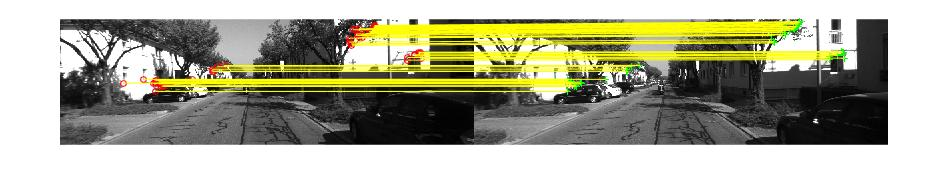
\includegraphics[width=0.98\textwidth]{files/KLT_2d2d.jpg}
\caption[2D-2D Correspondences with KLT]{\label{fig:KLT_2d2d}2D-2D Correspondences with KLT.}
\end{figure}

An examplary output of the 2D-2D module can be seen in Figure~\ref{fig:KLT_2d2d}. The correspondences between two images are indicated.

Due to efficiency reasons we decided to use the epipolar line distance as a measure to validate the estimated Fundamental Matrices. In theory the reprojection error would have yielded better results (sacrificing efficiency); however, in our case the differences were neglectable.

\section{Continuous Operation}
\label{s:ContOp}

\subsection{KLT}

\section{Bonus Features}
\label{s:BF}

\subsection{Plotting}
The source code provides extensive plottings to help debug the pipeline. These are enabled by using the $debug\_with\_figures$ flags
on the different modules of the pipeline. Moreover, in order to properly visualize the logic of the pipeline, we show a Figure 
with the main output of the odometry estimation. \\
At the top left of the mentioned Figure, it is shown the current frame that is being processed. On top of it we plot the keypoints
triangulated in green, while in yellow we plot the ones that have not yet been triangulated but are potentially going to be
triangulated. \\
The figures below the image present both the number of landmarks that are being tracked (left image) and the global trajectory
estimated by the algorithm. \\
Finally, the figure on the right shows the last poses of the camera together with the last triangulated landmarks.


\subsection{Automatic Selection of Frames for Initialisation}
We have further implemented the Bonus Feature "Automatic Selection of Frames for Initialisation". The initialisation will try to find correspondences between different frames in the beginning of the datasets. If a pair of initialisation candidates has enough correspondence inliers the automatic selection tries to find the best pair which minimizes:

\begin{enumerate}
\item The average reprojection error and 
\item the average epipolar line distance.
\end{enumerate}

Once the minimizing pair was found, the monocular initialisation is recomputed with the new initialisation set of images.

\subsection{Relocalisation}
It can always happen in VO-pipeline that the errors introduced are getting to big and thus, localization is lost. In such a case, we need to be able to recover from the lost localization to further track the camera motion. \\
We have implemented a relocalisation state in the pipeline which covers this case. If the number of matched keypoints between two frames tends towards zero the track is lost. We reinitialise the track with two closeby frames with the help of the monocular initialisation. \\
However, the problem is that after reinitialisation also the scale gets reset. To counteract this we first need to recover the approximate scale where the track last ended. This scale is then reused after relocalisation. 

\subsection{Full Bundle Adjustment}

In our VO pipeline, we implemented two different approaches of bundle adjustment in order to refine the obtained pose estimates and landmark positions. The user can choose between different methods by setting the flag BA\_ to either ‘Offline’, ‘Online’, or ‘None’. 
BA\_ set to ‘Offline’ will perform full offline bundle adjustment to simultaneously optimize both, the trajectory of estimated poses as well as the 3D positions of triangulated landmarks, that have been recorded over a previously set number of frames. \\
This approach is based on the implementation provided with exercise 9. 

\begin{figure}
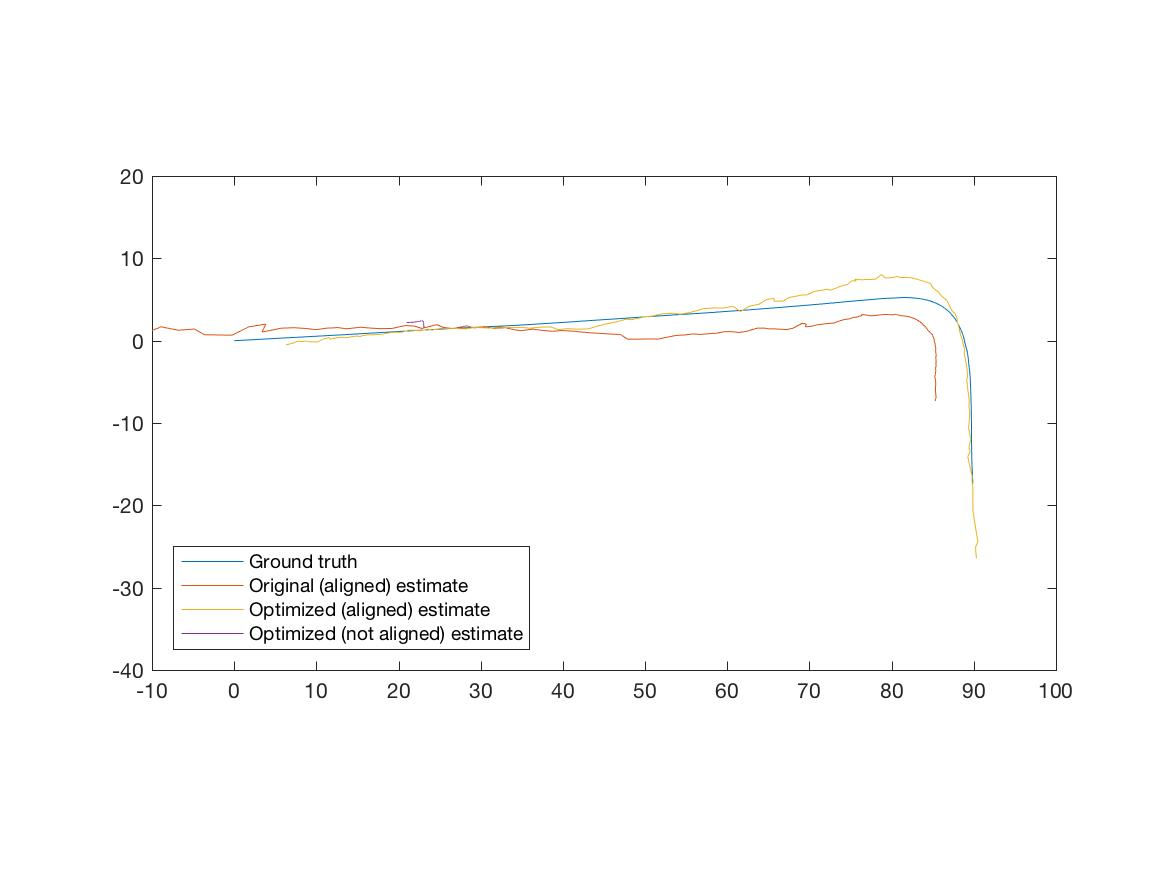
\includegraphics[width=0.99\textwidth]{files/aligned_optimized.jpg}
\caption[\label{f:aligned_optimized}Offline Bundle Adjustment]{This Figure shows the original estimated poses (orange) for the first 150 frames of the KITTI dataset. To account for the scale ambiguity of monocular VO, the obtained trajectory has been aligned to the ground truth by means of a similarity transformation.}
\end{figure}

If \textit{BA\_} is set to ‘Online’ full online bundle adjustment on a certain number of (key-)frames is performed to update the current pose estimate and the landmark positions observed in the last m frames. However, as can be seen in \textit{Video 5 – Online BA}, the code is not working properly in the sense of meaningfully improving the current pose estimate. The idea is that the poses, triangulated landmarks, and observed keypoints of the last m frames are stored and can be passed in the format introduced in exercise 9 to Matlab’s \textit{lsqnonlin} solver which then iteratively adjusts the last m poses and the positions of landmarks observed in those m frames by minimizing the reprojection error.  



\subsection{Calibrated Smartphone Camera and Own Dataset}

In order to assess the robustness of our VO pipeline, we decided to record our own dataset.
For this endeavour, we printed a checkerboard to calibrate the camera of an smartphone.
We then used the calibrated camera to record the dataset.
In order to achieve good results for the calibration, we made sure that we followed the following procedure:

\begin{enumerate}
	\item Set focus and exposure mode of the smartphone to fixed.
	\item Ensure that the checkerboard is over a planar surface and presents no light reflections.
	\item Take frames of the checkerboard from sufficiently different angles and distances.
\end{enumerate}

Once the calibration dataset recorded, we proceeded to find the intrinsics of the camera.
As a first approach we used the \href{https://www.vision.caltech.edu/bouguetj/calib_doc/}{Matlab Toolbox}.
Unfortunately, we could not get good calibration results.
This was in part due to the fact that the interface requires you to click on the
corners of the checkerboard in the image, and therefore limits the amount of images you can process in a given time.
We also used OpenCV to retrieve the calibration matrix of the camera. Nonetheless, we found that the most user-friendly
calibration tool was the one offered as a Matlab app named Camera Calibrator.

Using this last tool, we managed to retrieve approximately the same intrinsic parameters independently of the calibration images.
Once calibrated, we processed the images to get a gray-scaled, resized and undistorted set of images. Then we fed the new
dataset to our VO pipeline and checked the results with our ground truth.
The ground truth was taken approximately with no special instrumentation other than a meter.

We encountered many problems while recording the dataset, to name a few: motion blur when moving, changes of illumination on the scene,
maintaining a constant focus, transferring images, having enough features on the scene, etc.

In the end, we found that monocular initialisation was having difficulties to output a sufficient amount of 2D-3D correspondences.
This led the continuous operation part to stop after two frames on average. The reprojection errors on the triangulated keypoints were of
the order of magnitude of tens of pixels, depending on parameters and bootstrap\_frames.

In the end, we learned about different tools available for camera calibration and about the difficulties of recording a satisfiable dataset
for visual odometry. Or seen from another perspective, we learned about the limits of our VO pipeline.

Our calibration files and images of the dataset are provided under the folder smartphone.

\subsection{Quantitative Analysis}
\subsubsection{Keypoint Tracking via Block Matching versus KLT}

\begin{figure}
  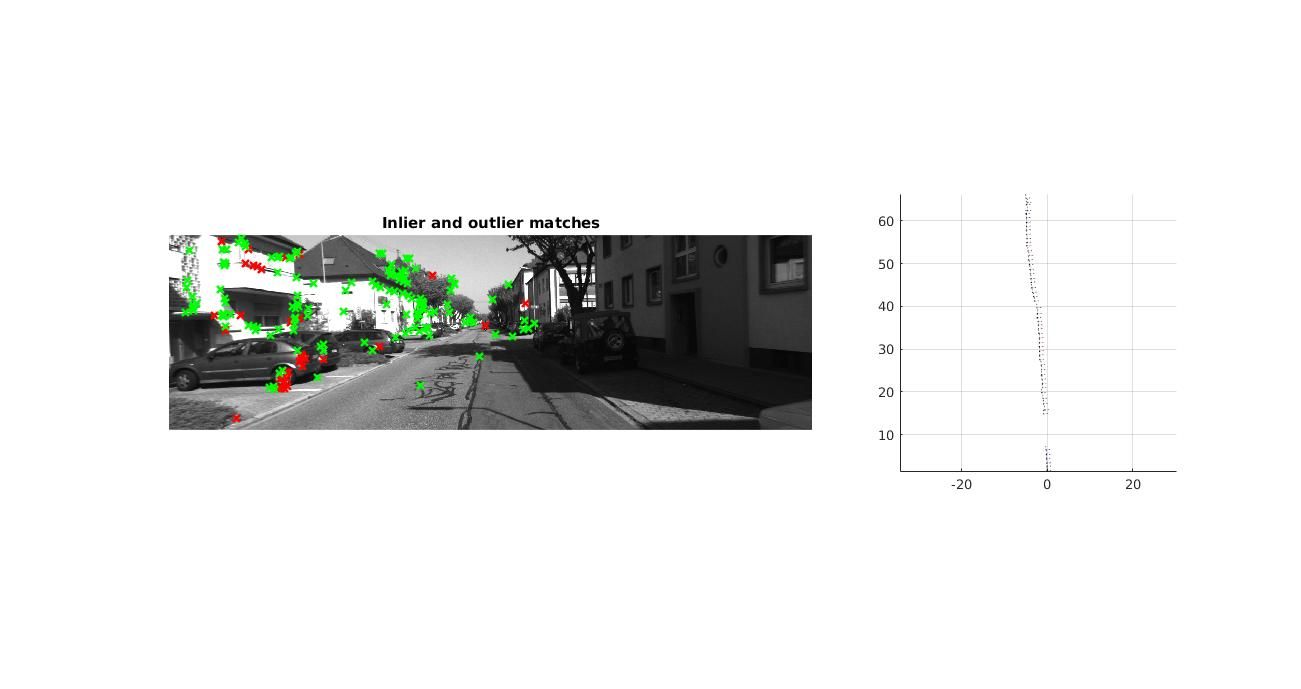
\includegraphics[width=0.99\textwidth]{files/block_tracker.jpg}
  \caption[Block Matching Tracker]{\label{f:block_tracker}Block Matching Tracker.}
\end{figure}

Our first approach to keypoint tracking was to implement a block matching algorithm. After describing the keypoints by a block of pixels around it we simply computed the sum of squared differences to match different blocks. This approach, while simplistic, performed reasonably well and we were able to actually localize reliably. As seen in this figure~\ref{f:block_tracker}, Block Matching gives overall good results but fails to track some keypoints. \\
Nonetheless, knowing that the range of movement is constrained in our datasets (small translational displacements) we thought that it would be appropriate to use a more performant tracker in this situations such as the KLT algorithm.

\begin{figure}
  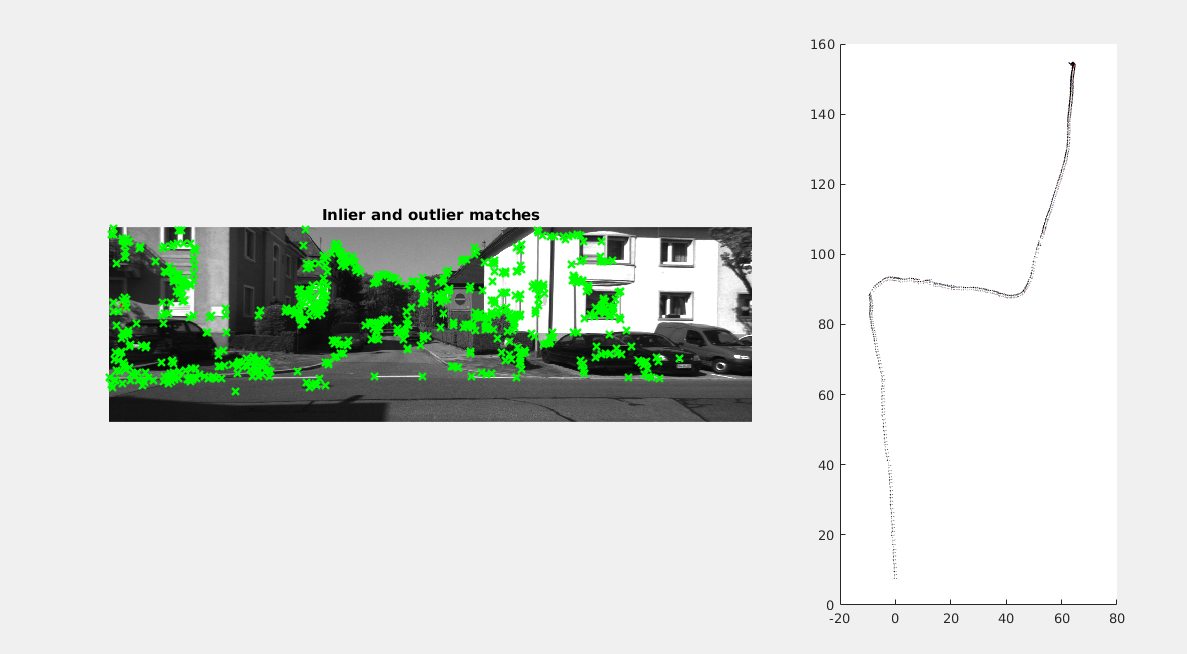
\includegraphics[width=0.99\textwidth]{files/klt_tracker.png}
  \caption[KLT Matching Tracker]{\label{f:klt_tracker}KLT Matching Tracker.}
\end{figure}


The simple replacement of the Block Matching algorithm by the KLT algorithm offered an overall better performance of the estimation due to its sub-pixel accuracy when tracking keypoints. As reference, this figure~\ref{f:klt_tracker} shows the performance of the KLT algorithm on the estimation of the pose.

\subsubsection{Analysis of performance of different ways to extract Harris features}

Extracting keypoints from the images is one of the most important parts of a visual odometry pipeline. For that reason, we
decided to do a quantitative analysis of the performance of the way we used the Harris detector. \\
In our implementation we added four different methods to apply Harris.
The first consists in an implementation that we believed could improve the performance of the keypoints extraction.
While running the pipeline we noticed that the keypoints were not uniformly detected over the image. \\
In order to get a more uniform set of keypoints over the image we decided to divide the frame into sub-images. We will refer to them
as bins. In each of these bins we run the Matlab implementation of "detectHarrisFeatures".

\begin{figure}
  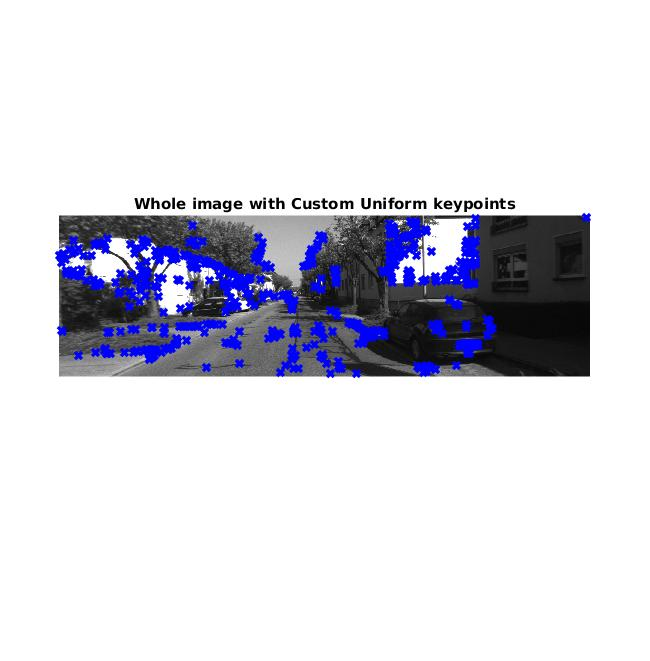
\includegraphics[width=0.99\textwidth]{files/custom_uniform_keypoints.jpg}
  \caption[\label{f:custom_uniform}Uniform Harris Implementation]{Uniform Harris Implementation.}
\end{figure}

\begin{figure}[b]
\subfigure[\label{f:strongest}Strongest Harris Features.]{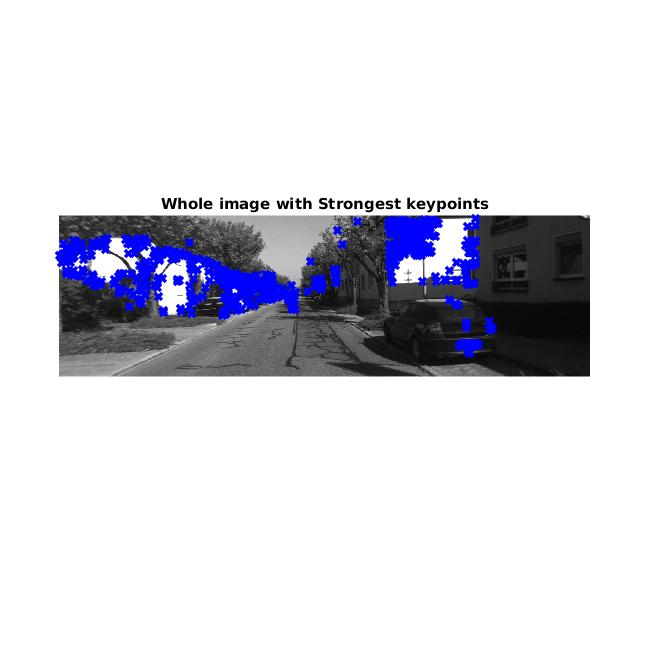
\includegraphics[width=0.49\textwidth]{files/strongest_keypoints.jpg}}
\subfigure[\label{f:custom_uniform}Uniform Harris Features.]{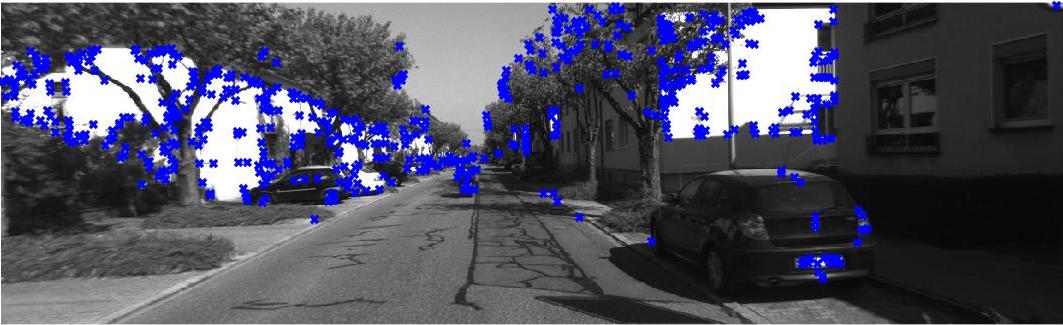
\includegraphics[width=0.49\textwidth]{files/uniform_keypoints.jpg}}
\caption[Harris Features]{\label{f:harris}Harris Features.}
\end{figure}

This provides us with localy optimal corners in
the bin. Applying this approach recursevely over the bins gives us an homogeneous extraction of features of the image. Figure~\ref{f:custom_uniform} 
presents the result of this implementation on the first frame of the Kitti dataset.

The other two algorithms that we may use consist in running the Harris corner detector over the whole image, as it is usually done. They differ between them in that one selects the strongest detected keypoints while the other selects them more uniformly. As it can be seen in Figure~\ref{f:strongest} and Figure~\ref{f:custom_uniform}, the uniform selection of keypoints performed by Matlab is still not homogeneous over the image.
This should not be a problem if the quality of the corners is good. \\ Nonetheless, we experienced in practice that a mapping of keypoints on different
patches of the image gives overall better results and is more robust to occlusions.